\section{Experiments}
% \begin{figure*}
%     \centering
%     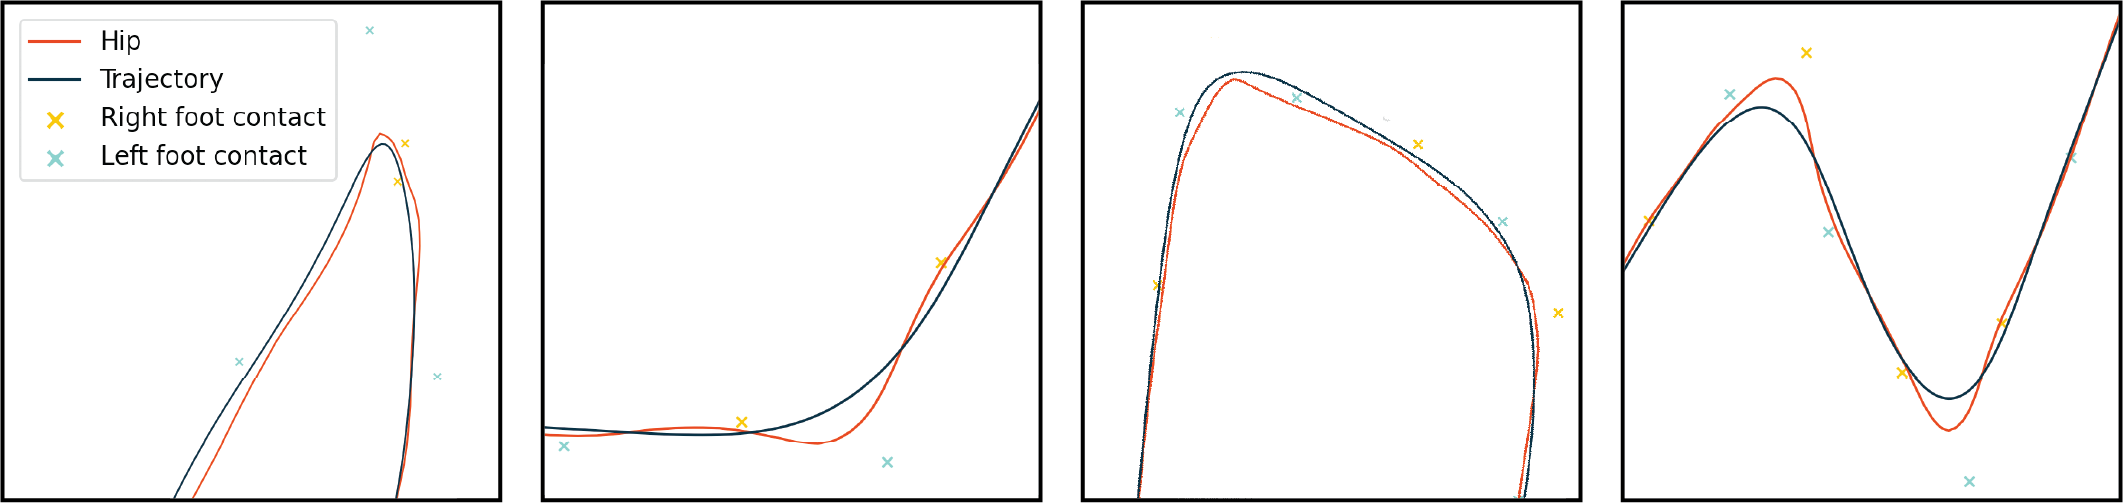
\includegraphics[width=1.0\linewidth]{img/estimated_trajectory_examples.png}
%     \caption{Top down view of 4 animation clips. Hip movement shows oscillations on straight paths and counter steering during turns. Estimated trajectories are cleaner and corresponds well with overall movements in the animations while excluding unnecessary details of to human locomotion characteristics.}
%     \label{fig:results:estimatedtrajectory:examples}
% \end{figure*}

\begin{figure}
    \centering
    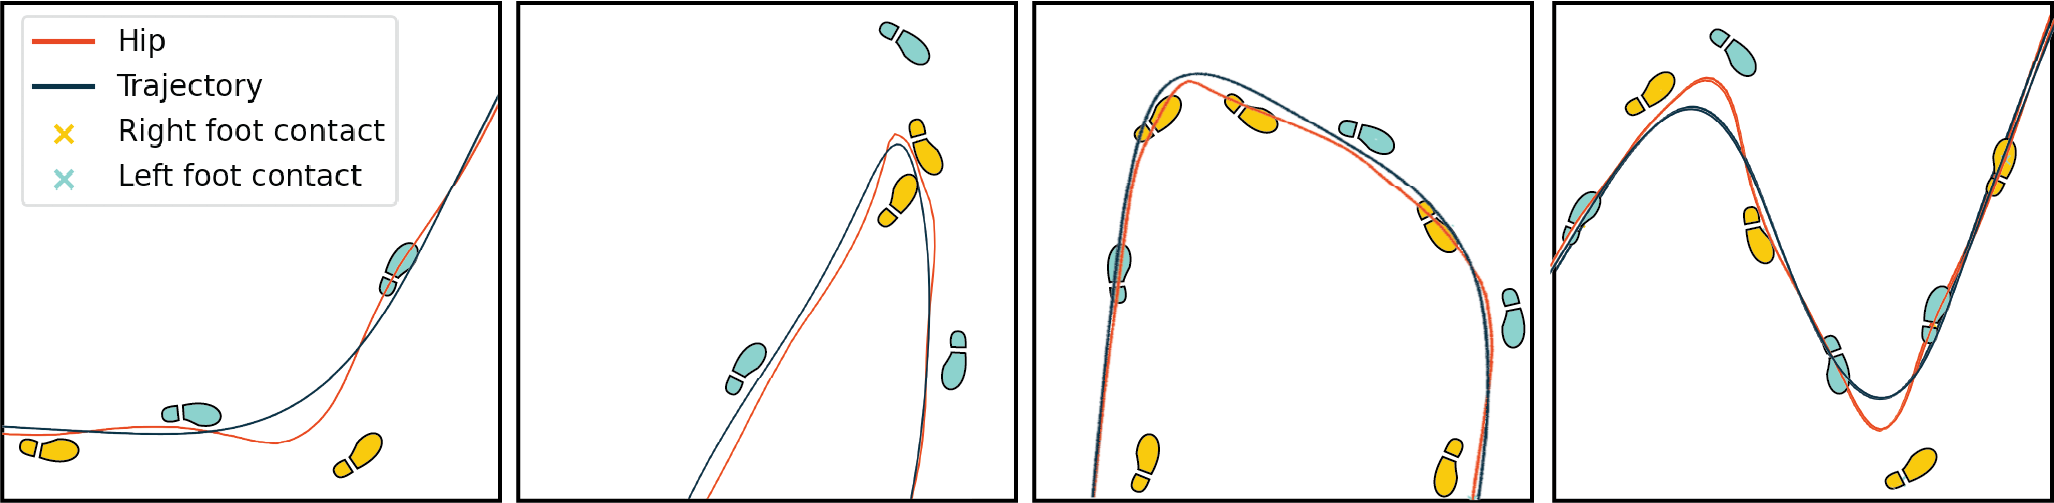
\includegraphics[width=1.0\columnwidth]{img/estimated_trajectory_examples_small.png}
    \caption{Top down view of 4 animation clips. Hip movement shows oscillations on straight paths and counter steering during turns. Estimated trajectories are cleaner and corresponds well with overall movements in the animations while excluding unnecessary details of to human locomotion characteristics.}
    \label{fig:results:estimatedtrajectory:examples}
\end{figure}
\magnus{NOTE: Video: SHow animation using capsule movement with simple exponential decay and original animations . Does not look nice. Then our solution}
We recorded a series of animations with the XSens inertial sensor suit on 3 different actors. The raw sensor data was cleaned using post processing available in the XSens MVN Animate Pro software. We recorded movements typically seen in 3rd person computer games by following industry standard 'dance cards', which are lists of movements that in total covers the expected range of motion of the player character. This style of animation differs from unstructured animation by having clearly defined segments such as 'forward-run' or '$45^o$-degree-walk-turn'. In a production setting the dance cards animation will usually be carefully cleaned and aligned by hand, but since our method addresses exactly those steps we analyze the raw animation data. As seen in the video some artifacts are present in the source recordings due to the lack of clean up.

\subsection{Trajectory Estimation}
We estimate trajectories by connecting foot contact center points as described earlier. We detect foot contacts by manual tuning of threshold values for speed and height of the feet. In our experience globally valid thresholds are easily found, since only a single start-contact point is needed without great precision.Overall the method works well, and is robust to the movements seen in our animations. Examples of the estimated trajectories are plotted against ground projected hip movement in Fig. \ref{fig:results:estimatedtrajectory:examples} and the detected foot contacts are marked. While it is challenging to quantify the quality of the estimates we notice several desirable properties such as a lack of oscillations on straight segments and turn curves with tangents similar to the general direction of movement. Fig. \ref{fig:results:estimatedtrajectory:stats} further illustrates that changes in direction (as indicated by spikes in the angular velocity plot) show a clear pattern  which is not evident in the hip movement alone. As such the hip or center of mass movement can be seen as trajectories occluded by a noise component due to human locomotion characteristics. Notice how the hip movement shows repeated and opposite angular velocities for each foot contact, while our trajectories have either no changes or spikes without a pattern, where the latter indicates natural corrections done by the actor to stay on a straight line. 

To avoid sharp trajectory changes on foot contacts we apply a gaussian filter with a constant standard deviation in a $0.1$ second window around each contact. This filtering is not applied to remove noise from the signal as in traditional trajectory estimation techniques and does not require any tuning as long as the window size is kept smaller than the distance between consecutive foot contacts. The effect is also shown in Fig.\ref{fig:results:estimatedtrajectory:stats}.   

\magnus{Maybe show 4 frames of an animated character with a capsule drawn on top to illustrate visual effect of consistent trajectory}
\magnus{Maybe show velocity profiles ? Ie we not have smooth movement, but also smooth velocities/ constant acellerations}

\begin{figure}
    \centering
    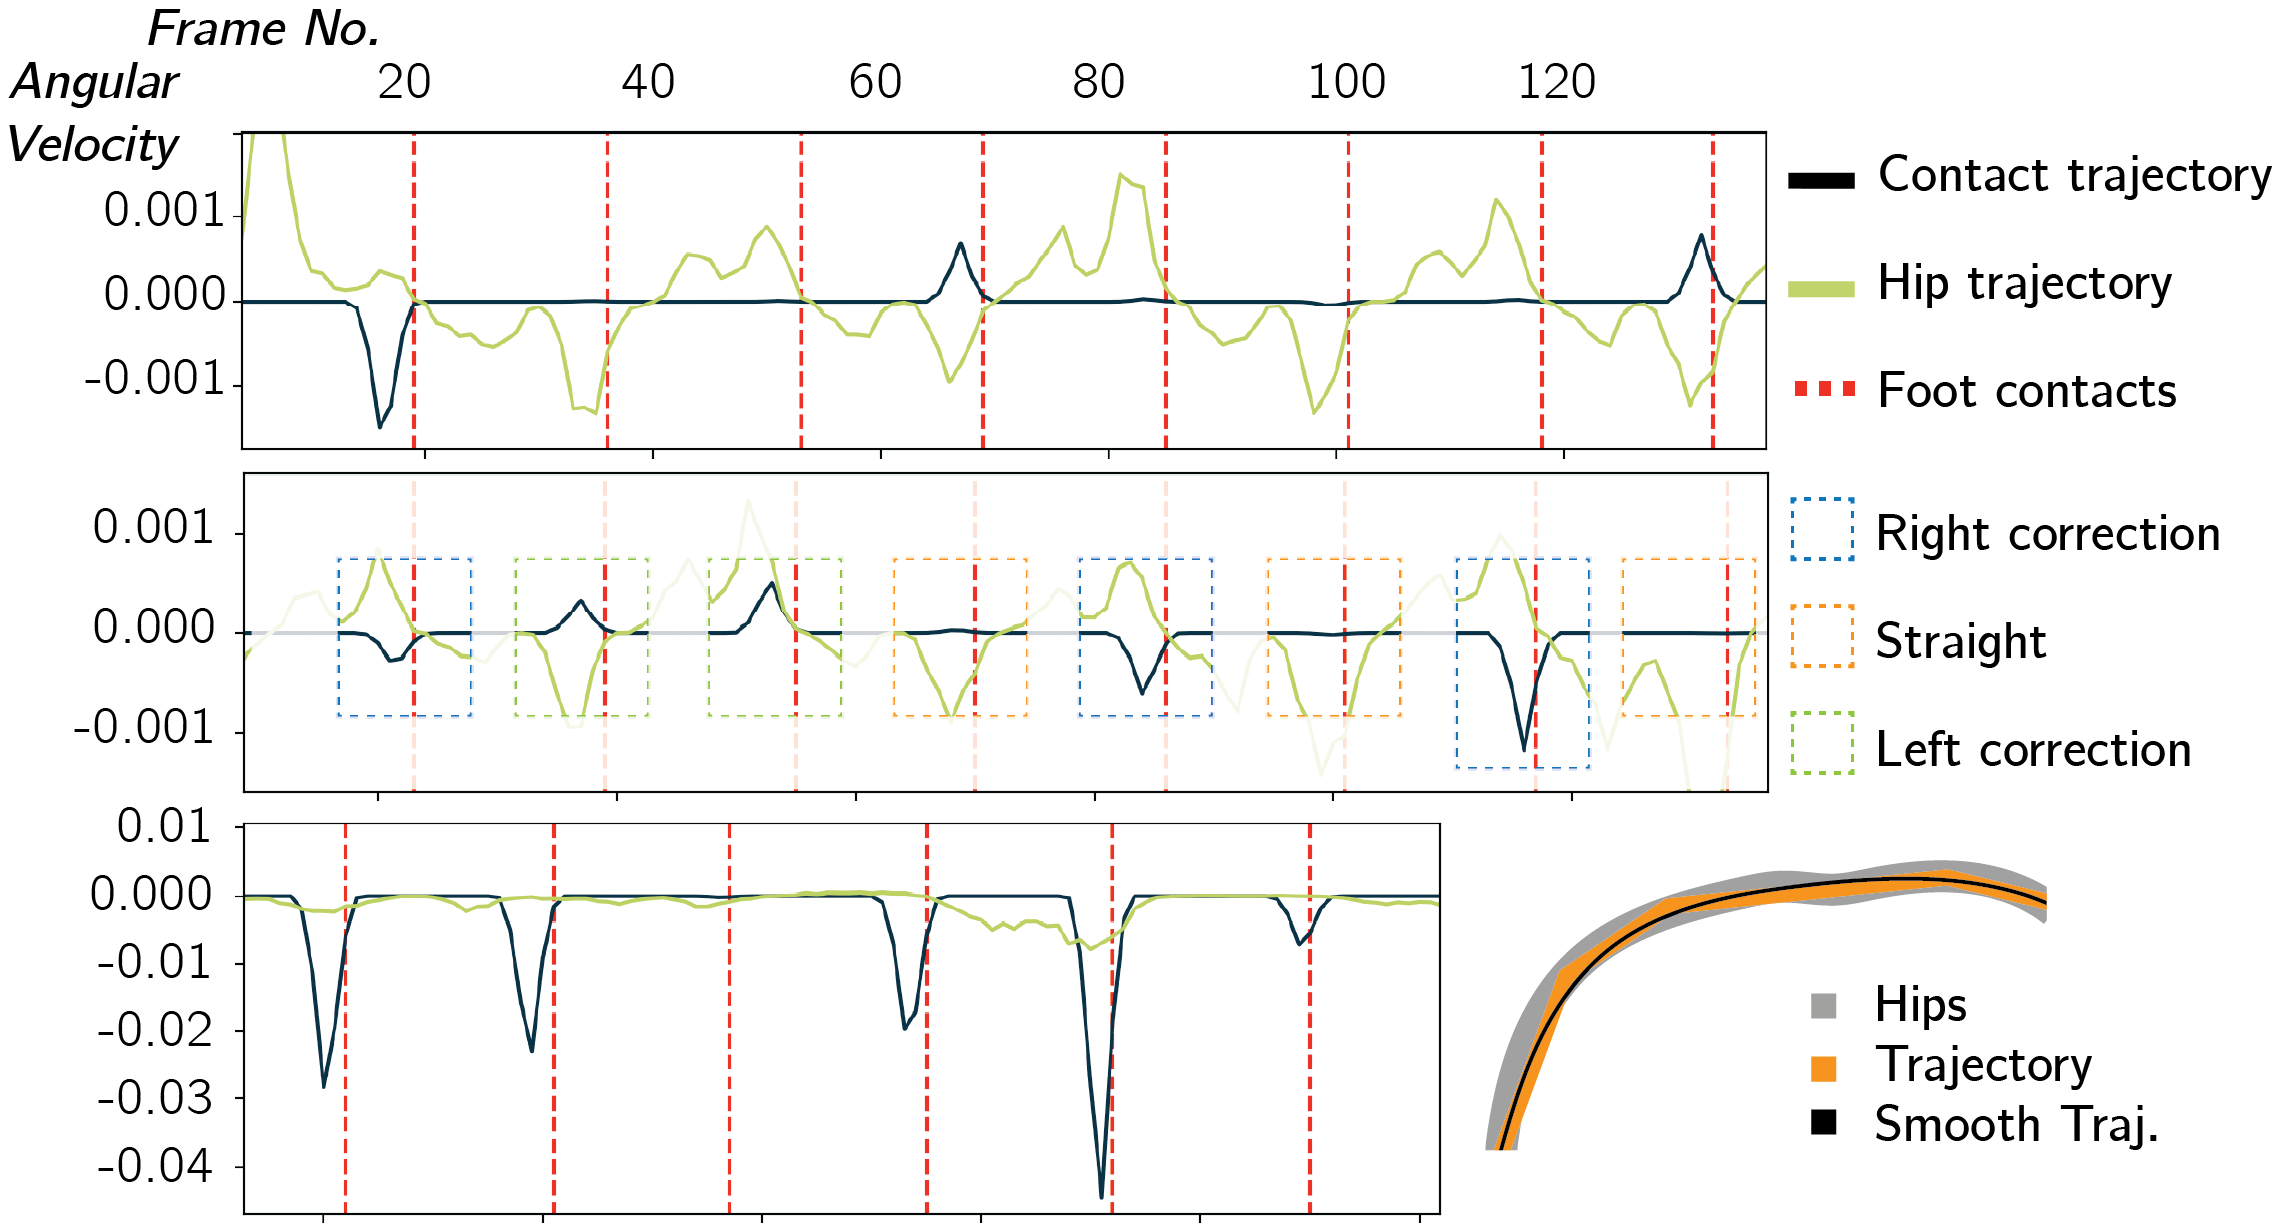
\includegraphics[width=1.0\columnwidth]{img/estimated_trajectory_angular_velocity.png}
    \caption{Angular velocity profiles of 3 animation clips. Top: Straight movement. Center: Straight movement with more adjustments to stay on path. Bottom: A turn. Estimated trajectories show clear peaks and smaller integrals of angular velocities compared to projected hip movement. Positive and negative angular velocities indicate right and left steering respectively. The estimated trajectories of straight animations show clear localized adjustments to heading, while hip movement obfuscate details.\\The bottom plot also shows the effects of applying local smoothing around foot contacts.}
    \label{fig:results:estimatedtrajectory:stats}
\end{figure}


\subsection{Control Genome extraction and movement alignment}
Our animations are based on dance cards with clearly defined regions and repeating straight-turning-straight segments. Turns are in the range from $0^o-180^o$ and we captured a variation of both walking and running from our 3 actors. The clear patterns makes it easy to extract reduced control genomes where an initial position and velocity pair is combined with directions offset in time. Fig. \ref{fig:results:genome_extraction} illustrates how a control genome is extracted from a single left turn using a simple heuristic. If more complex animations are used we imagine that statistics of recorded stick movements during gameplay or manual annotation could be used to construct control genomes. 
\begin{figure}
    \centering
    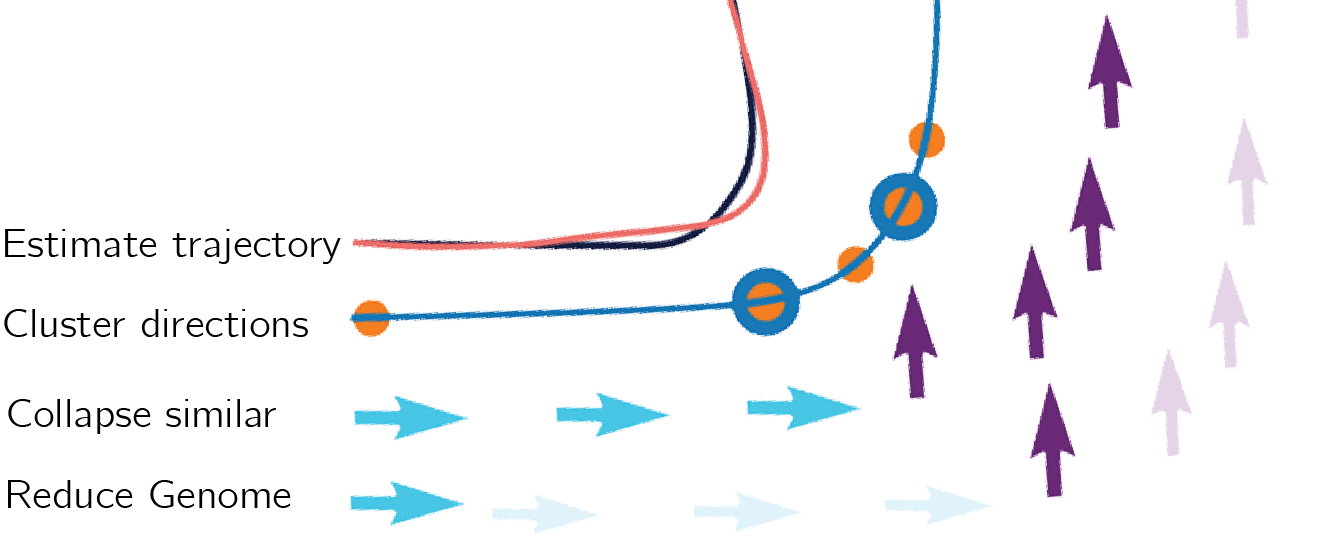
\includegraphics[width=1.0\columnwidth]{img/genome_extract.png}
    \caption{Control Genome is extracted from an animation where the actor runs forward then does a left turn and runs straight again. We extract an initial position, velocity and facing direction at the positions of the turquise arrow. And then control direction and time offsets at the position of the both the turquise aand purple arrow.}
    \label{fig:results:genome_extraction}
\end{figure}

After genome extraction we defined straight animation sections to begin when the animation velocity is parallel with the current control genome direction, and end when a new direction is encountered as previously described. Each straight segment is fitted to remove minor divergences from the straight line.
% \begin{figure}
%     \centering
%     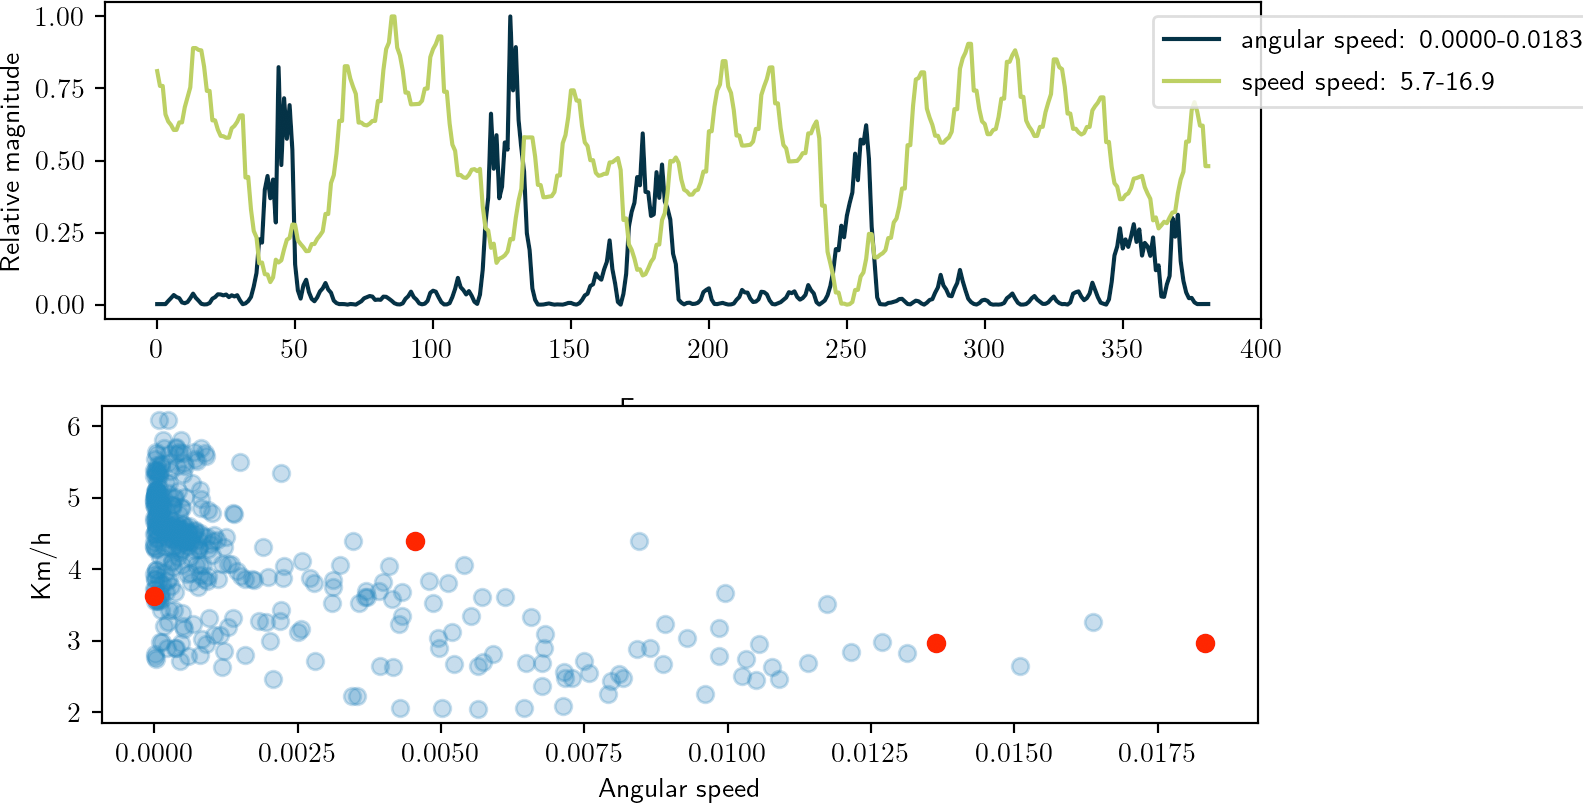
\includegraphics[width=1.0\columnwidth]{img/movement_stats.png}
%     \caption{An animation with 5 90 degree turns has complex changes to speed and angular speed.}
%     \label{fig:results:trajectory_estimation}
% \end{figure}
% \begin{figure}
%     \centering
%     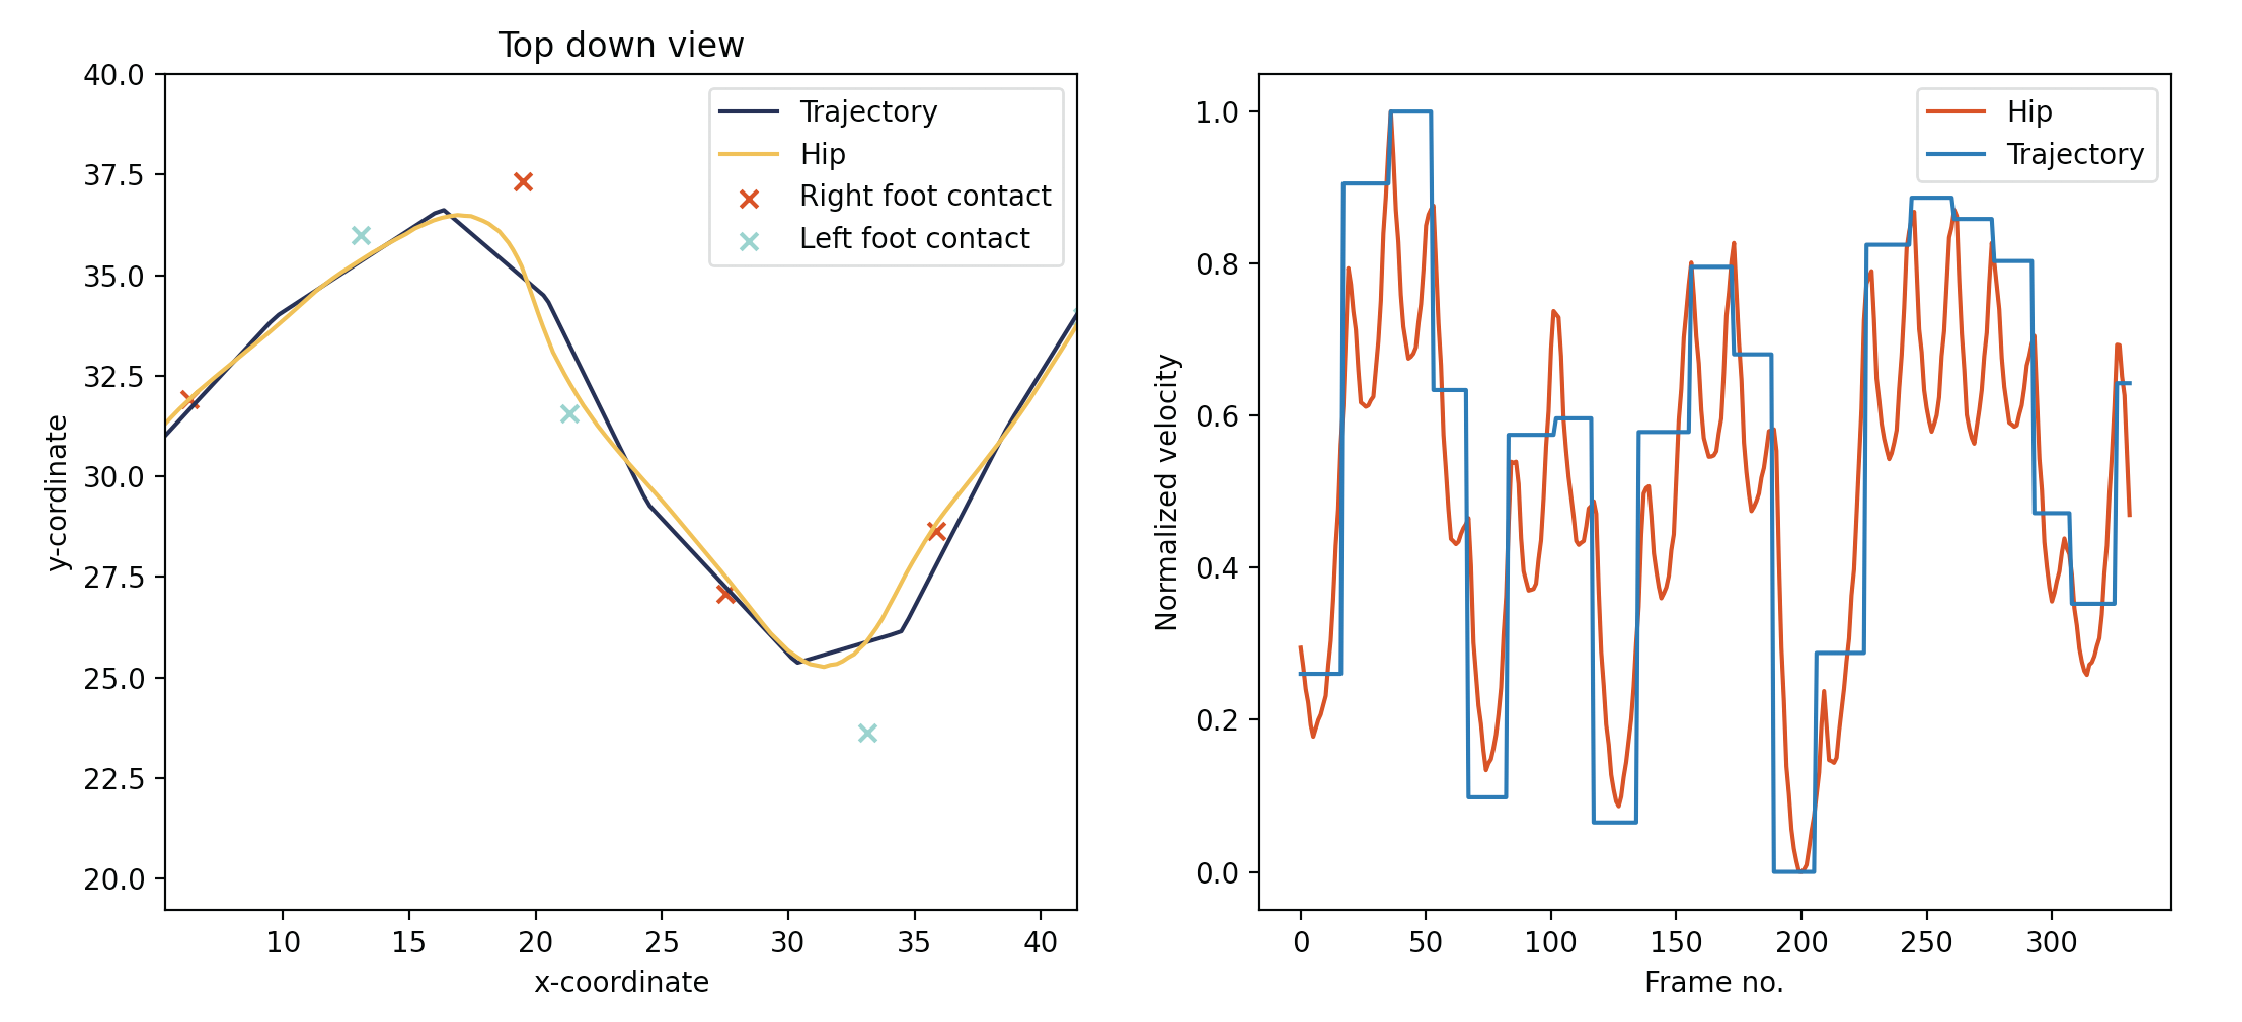
\includegraphics[width=1.0\columnwidth]{img/trajectory_estimation.png}
%     \caption{Left plot shows hip movement cross back and forth between the estimated trajectory, and tangential directions sampled at individual positions hip give poor descriptions of the overall movement direction. Right plot show trajectories having more stable velocities.}
%     \label{fig:results:trajectory_estimation}
% \end{figure}

% \begin{figure}
%     \centering
%     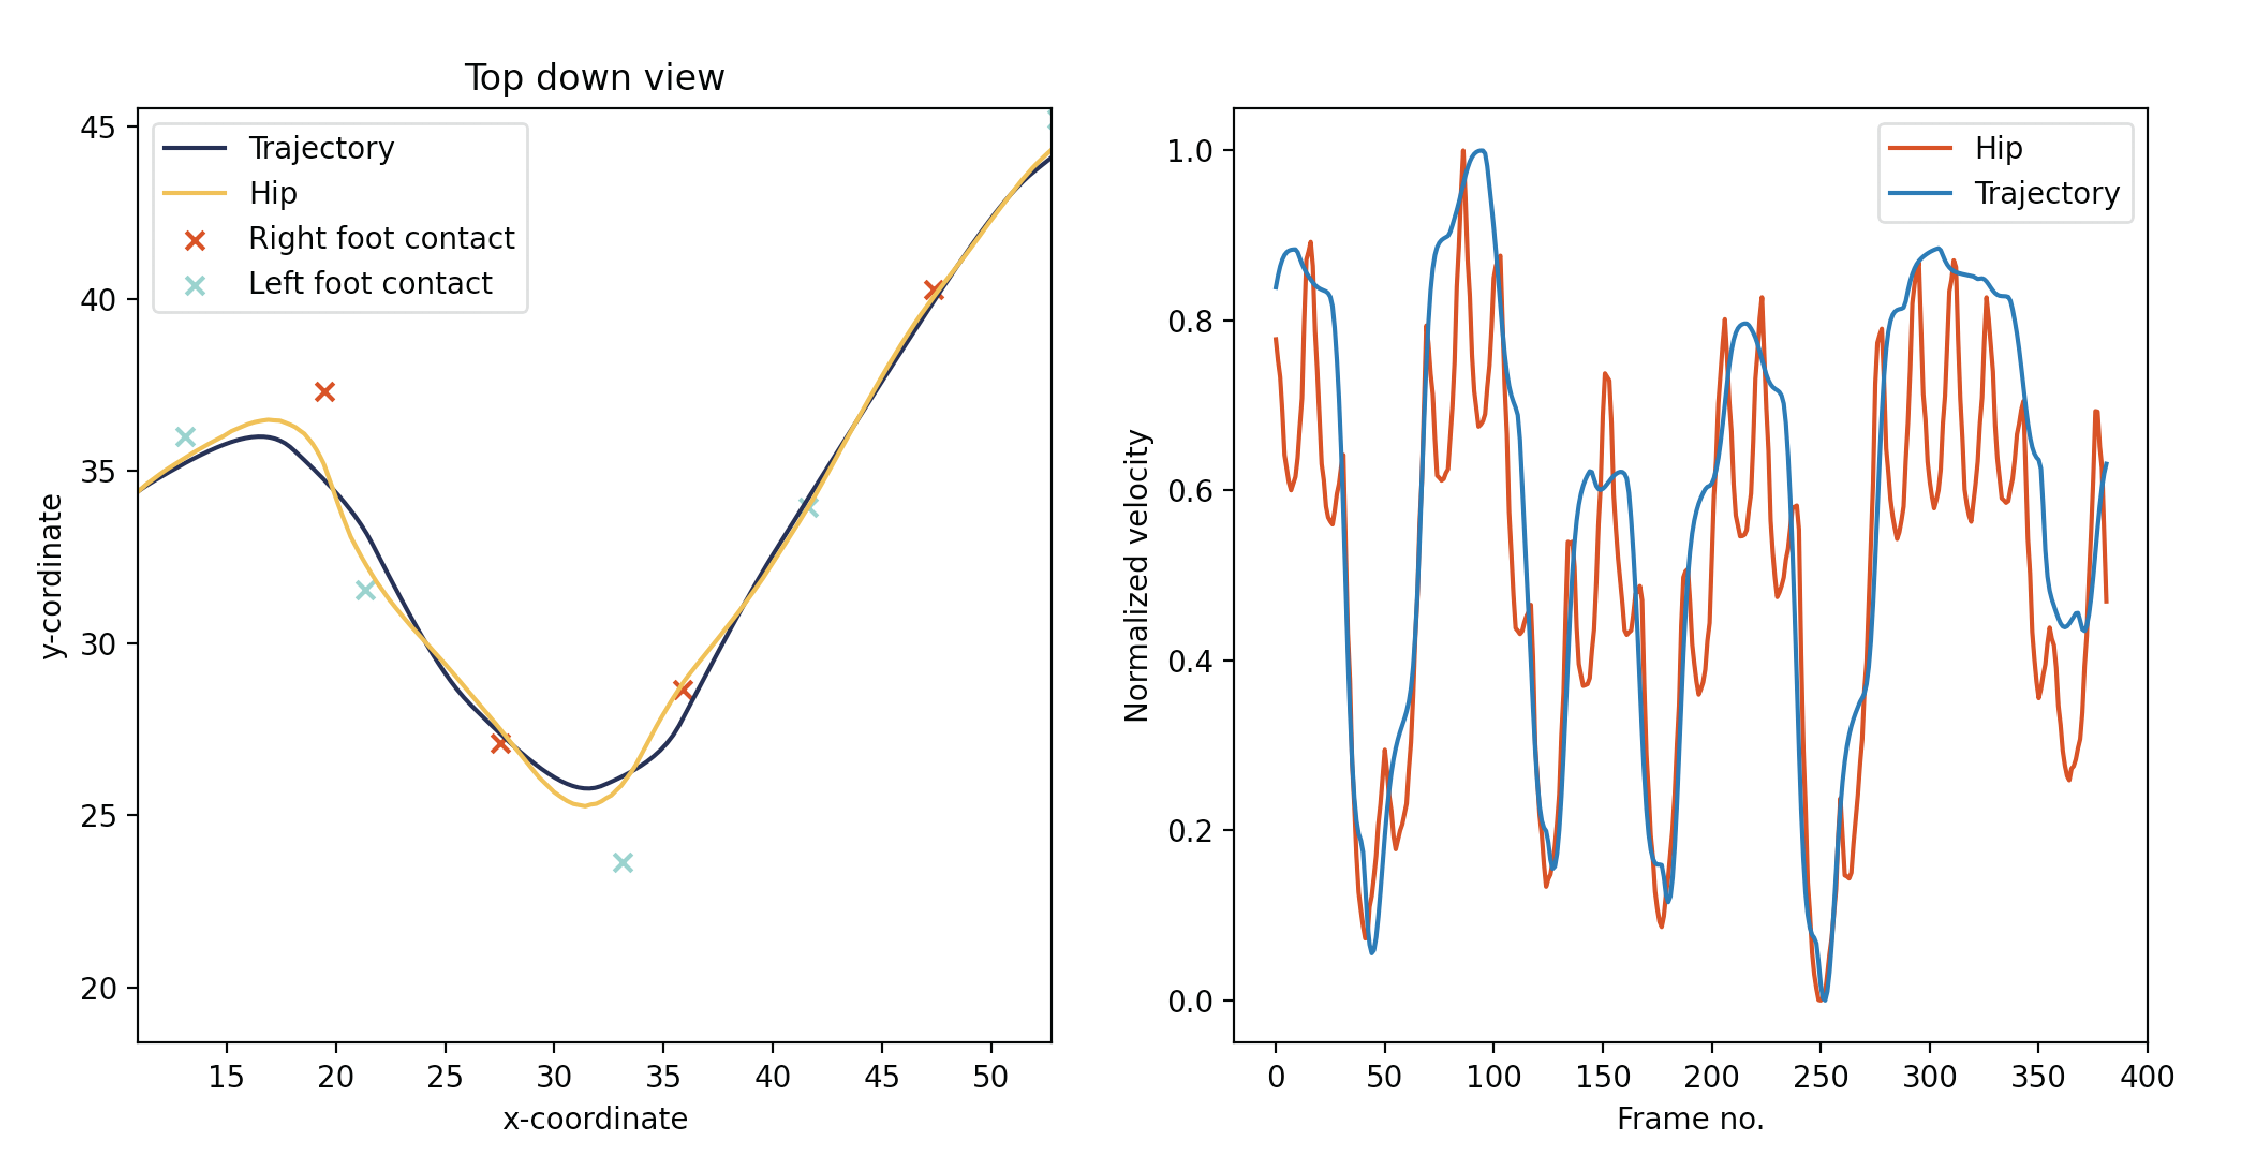
\includegraphics[width=1.0\columnwidth]{img/trajectory_estimation_smooth.png}
%     \caption{By interpolation frame delta across foot contact dependent section, we achieve a smoother sampling of the trajectory. The smoothing is visible in both the path and the velocities.}
%     \label{fig:results:trajectory_estimation_smooth}
% \end{figure}

% \begin{figure}
%     \centering
%     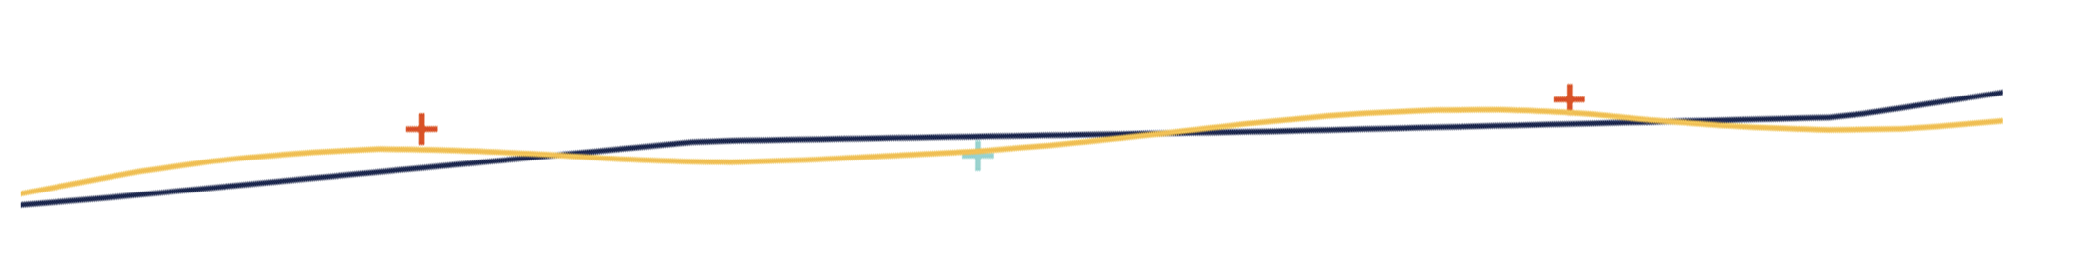
\includegraphics[width=1.0\columnwidth]{img/straight_trajectory.png}
%     \caption{}
%     \label{fig:results:trajectory_straight}
% \end{figure}
\subsection{Movement Model Fitting}
We performed local fittings on our animations using control genomes with 2-5 changes in direction. The optimization was performed using PyTorch and the Adagrad optimizer with a learning rate of 0.1. Convergence rates are shown in Fig. [??] and visual examples in Fig. \ref{fig:results:engine_view} and the supplied video material. Our model is able to reproduce relatively complex motion planning such as a gradual slow down in speed before starting to rotate during a $180^o$ turn and two phase accelerations during softer turns using only 17 adjustable parameters. 

\magnus{Convergence, increase genome count}



As more direction are added the error accumulates along the path, 
\begin{figure}
    \centering
    \includegraphics[width=1.0\columnwidth]{img/engine_view.png}
    \caption{OMG}
    \label{fig:results:engine_view}
\end{figure}

% \subsubsection{Automated Control Genome extraction}
% Automated genome extraction is shown in Fig. \ref{fig:results:genome_extraction}.
% \subsubsection{Alignment}
% \subsubsection{Fitting}

% \subsection{Global Fitting}

% \begin{figure}
%     \centering
%     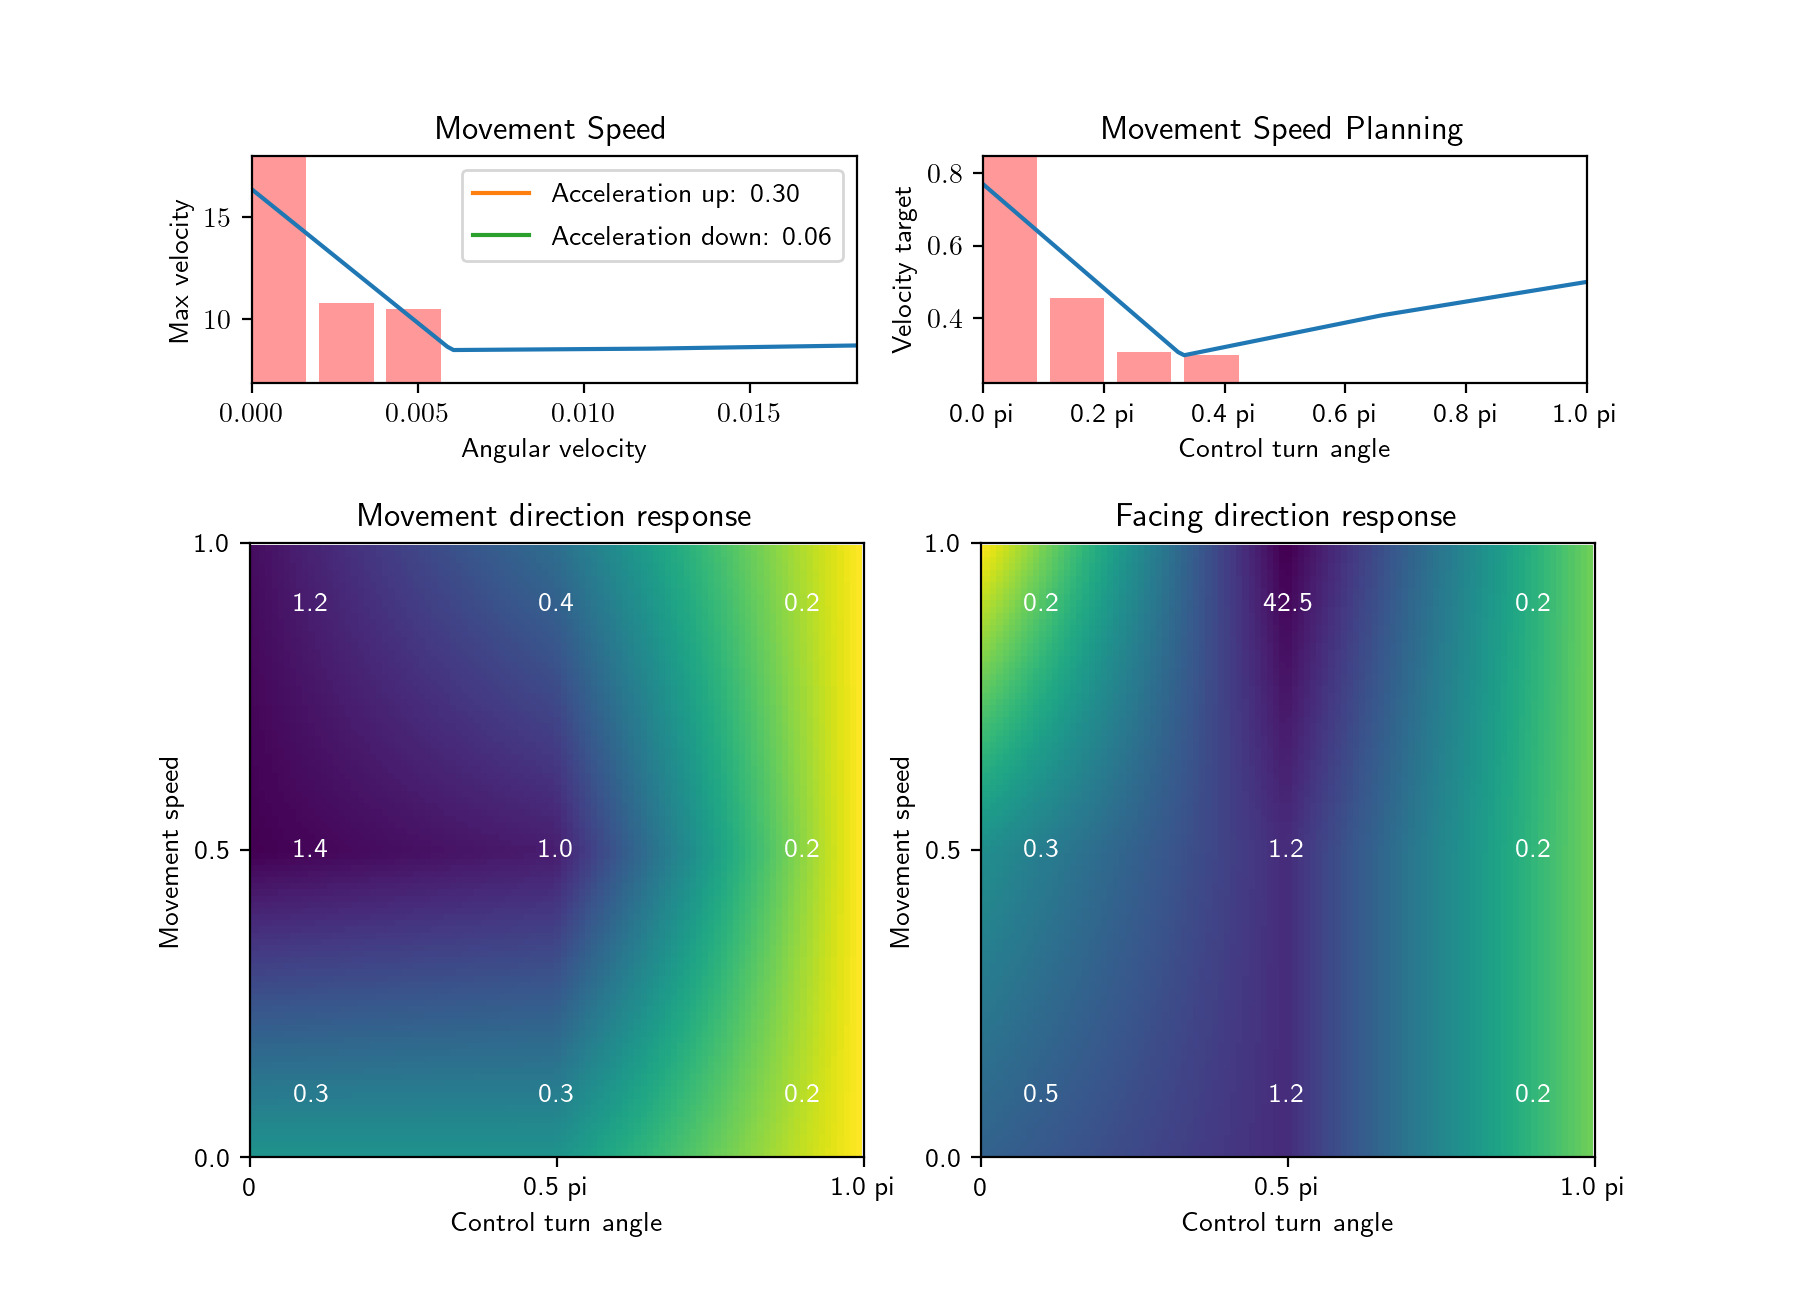
\includegraphics[width=1.0\columnwidth]{img/locomotion mode.png}
%     \caption{}
%     \label{fig:results:locomotion_mode}
% \end{figure}



% \section{Video Notes}

% \subsubsection{Purpose}
% Illustrate the problem we wish to solve using 1-2 video examples.
% \subsubsection{Content}
% Show that basic animations have complex root motions that are difficult to replicate using standard 'weak control signal' (splines, springs). 
% Show that trivial approaches (smoothing) does not solve problem in convincing way.
% \paragraph{Videos}
% \begin{itemize}
%     \item Show character moving straight and in curves. Trace complex root motion. Highlight the presence of both high and low frequency information in the plot.
%     \item Show character running straight with smoothed trajectory. Highlight problems. Show turning characters and illustrate how superficially 'identical' turns are actually very different.
% \end{itemize}
% \paragraph{Figures}
% \begin{itemize}
%     \item Plots of trajectory and weak control signal paths.
%     \item Plots of smoothing effects
% \end{itemize}

% \subsubsection{Draft}
% Final text

% \subsection{Fitting Movement Model}
% \subsubsection{Purpose} Show that we are able to solve problem using 3-5 video examples (didactic).
% Show how various models can be fitted to data (that has itself been adjusted). 
% \begin{itemize}
%     \item Straight movement. Walk and run. 
%     \item Multiple straight movements. Walk and run. 
%     \item 180.
%     \item Multiple 180s.
%     \item Banking
%     \item Multiple banking
%     \item 45 turn
%     \item Multiple 45 turn
%     \item 90 turn
%     \item Multiple 90 turn
%     \item Mixed modes
% \end{itemize}
% Additionally we could look at animations published by ubisoft.\url{https://github.com/ubisoft/Ubisoft-LaForge-Animation-Dataset}


% \subsection{Global Fitting}

% \subsection{Application}
% \subsubsection{Purpose} Show that our solution has interesting applications using 3-5 video examples (eye candy).
% Replace standard control signal with our model.
% \begin{itemize}
%     \item{Replay animations to illustrate correct root motion}
%     \item{Use with motion matching} exponential decay = uttner, Holden Spring damper Kermse 2004].
%     \item{use generative neural network} Can we avoid floating character ?
% \end{itemize}

